\documentclass{article}
\usepackage[utf8]{inputenc}
\usepackage{listings}
\usepackage{graphicx}
\lstset{ %
frame=single, language=Java,breaklines=true,numbers=left,showspaces=false, showstringspaces=false,captionpos=b}
\title{OIS M2}
\author{Jolien Declerck, Silke Verhaeghe, Arno De Witte}
\date{8 March 2016}

\begin{document}

\maketitle

\section{Abstract}
We are building an application which allows the user to keep track of the amount of calories that he/she eats a day.  The application provides a way to track the desired amount of food the user should eat in order to stay on the same weight. Based on the amount of calories the user needs, some recipes are proposed. The user could provide a desired weight, which will lead to an adaptation of the needed calories intake.

\newpage

\section{Conceptual schema}



  \begin{figure} [h!]
     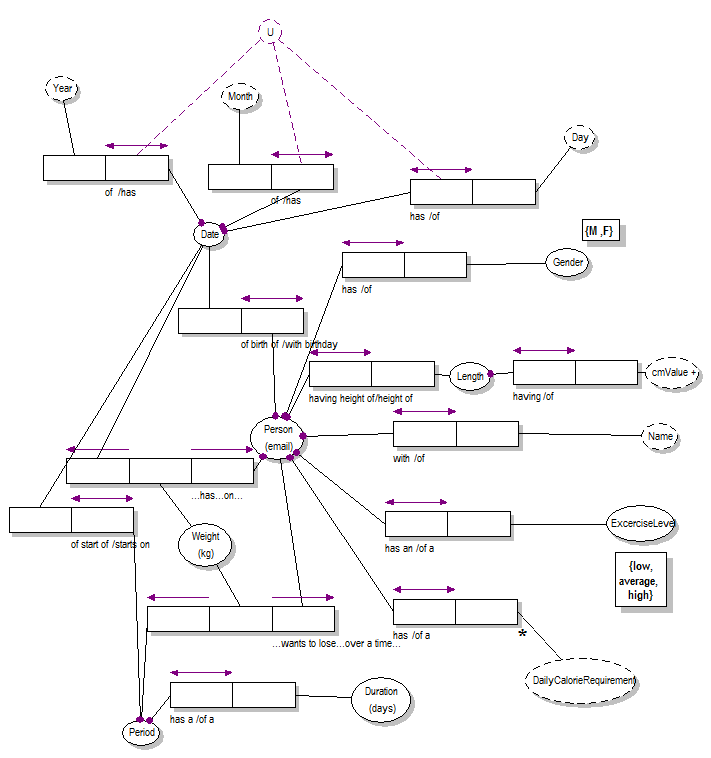
\includegraphics[width = 1.3\textwidth]{image/Person} 
     \caption{ORM of a person}
     \label{fig:twotier}
  \end{figure}


  \begin{figure} [h!]
     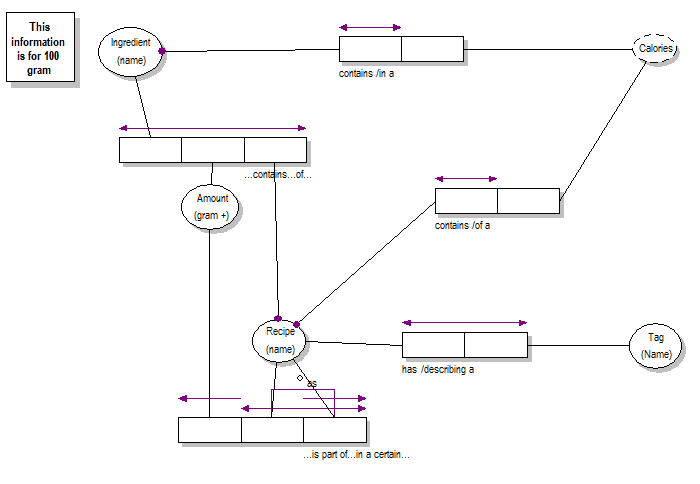
\includegraphics[width = 1.3\textwidth]{image/Recipe} 
     \caption{ORM of a Recipe}
     \label{fig:twotier}
  \end{figure}
\newpage

\subsection{Person} 

We base our application on a person which has as unique identifier an e-mail address. We provide basic information about the user like its  name, height in centimeters, gender, birth date. The gender of a user can be either female or male. A user has an exercise level, this can be high, low or average. This exercise level is important since the amount of calories a user needs in a day is dependant on the amount of exercise the person does. An active person will need a higher amount of calories in a day. Since the application needs to be able to show the fluctuation of the weight of a person, we keep track of how much a person weighs on a specific date. In order to calculate the daily amount of calories the user needs in order to stay on the same weight, we use the following formula: \newline
Basal Metabolic Rate (BMR) of a man= 10 * weight(kg) + 6.25 * height(cm) - 5 * age(y) + 5 \newline
Basal Metabolic Rate of a  woman = 10 * weight(kg) + 6.25 * height(cm) - 5 * age(y) - 161 \newline
In ordor to calculate the amount of calories a person needs we need to multiply this BMR with 1.3 if the exercise level of the person is light, multiply it with 1.6 if the exercise level is average and multiply it with 2.1 if the exercise level is high. The user's latest weight is used as the weight. This daily calorie amount is derived and not stored. A user also has the possibility to give a weight loss/gain amount, starting at a specific date for a period of days. Then the weight in the formula to calculate the needed calorie amount is adapted on the desired weight. 

\subsection{Ingredient}
The application has a list of ingredients, identified by their name. It also keep track of the amount of calories for 100 gram of the ingredient. An ingredient can be part of a recipe. In that case we also keep track of how much of the ingredient is needed.

\subsection{Recipe}
 A recipe has an amount of calories, which is the sum of all ingredients with their calories. Recipes can be easily found with a tag. This tag can be general and includes for instance breakfast but also more specific, for example; Chinese or Italian. A recipe can be part of another recipe for example the recipe for spaghetti sauce is part of the recipe for lasagna. In that case we also keep track of the amount of the recipe that is needed.   


\section{Database}
Based on this conceptual schema, a relational database schema was created. For this we used a MySQL relational database. In appendix 1 the SQL used to create the schema is given. As seen in the SQL statement, we used id's to create primary keys for the different concepts (person, recipe, ingredient and tag). This because it is more efficient and clearer to reference different concepts in the relation tables. These are then used as primary keys within the different relations among the concepts. In the persons table a few encodings are used. For one gender is marked by a single character m or f for either male or female. The level of exercise is encoded as an integer from low to high between 1 and 3.\\
A dump with test data is also included in the deliverables. 

\section{Application layer}
The application layer should be able to calculate the daily calorie requirements and a user should be able to keep track of how much calories he/she already had that day. It should be able to show a user a graph of his/her weight fluctuations.It should be able to adapt the calorie needs of a user according to it's desired weight. The application layer can recommend the user some recipes according to the calorie needs the user has.

\section*{Appendix}
\subsection*{Appendix 1}
\begin{lstlisting}[caption=Script of database]
CREATE TABLE  IF NOT EXISTS `persons` (
person_id INTEGER UNSIGNED AUTO_INCREMENT PRIMARY KEY,
name VARCHAR(20) NOT NULL,
length INTEGER(3) NOT NULL,
gender VARCHAR(1) NOT NULL, /* 'm' for male, 'f' for female*/
birthdate DATE NOT NULL,
excercise_level INTEGER(2) NOT NULL, /* 1 low, 2 average, 3 high */
email VARCHAR(50) NOT NULL, /* Possibly more emails in the future */
CONSTRAINT uniquePerson UNIQUE (email) /* No 2 users with the same email */
) ENGINE=INNODB;

CREATE TABLE IF NOT EXISTS `looses_weight` (
    person_id INTEGER UNSIGNED,
    period INTEGER,
    start_date DATE,
    weight_to_lose INTEGER NOT NULL,
    CONSTRAINT looses_pk PRIMARY KEY (`person_id`, `start_date`, `period`),
    FOREIGN KEY (person_id) REFERENCES `persons`(person_id) ON DELETE CASCADE
) ENGINE=INNODB;

CREATE TABLE IF NOT EXISTS `person_weighs` (
    person_id INTEGER UNSIGNED,
    on_date DATE,
    weight INTEGER NOT NULL,
    CONSTRAINT weighs_pk PRIMARY KEY (`person_id`, `on_date`),
    FOREIGN KEY (person_id) REFERENCES `persons`(person_id) ON DELETE CASCADE
) ENGINE=INNODB;

CREATE TABLE IF NOT EXISTS `recipes` (
    recipe_id INTEGER UNSIGNED AUTO_INCREMENT PRIMARY KEY,
    name VARCHAR(20) NOT NULL,
    calories INTEGER NOT NULL
) ENGINE=INNODB;

CREATE TABLE IF NOT EXISTS `ingredients` (
    ingredient_id INTEGER UNSIGNED AUTO_INCREMENT PRIMARY KEY,
    name VARCHAR(20) NOT NULL,
    calories INTEGER NOT NULL
) ENGINE=INNODB;

CREATE TABLE IF NOT EXISTS `tags` (
    tag_id INTEGER UNSIGNED AUTO_INCREMENT PRIMARY KEY,
    name VARCHAR(20) NOT NULL
) ENGINE=INNODB;

CREATE TABLE IF NOT EXISTS `recipe_tag` (
    recipe_id INTEGER UNSIGNED,
    tag_id INTEGER UNSIGNED,
    CONSTRAINT recipe_tag_pk PRIMARY KEY (`recipe_id`, `tag_id`),
    FOREIGN KEY (recipe_id) REFERENCES `recipes`(recipe_id) ON DELETE CASCADE,
    FOREIGN KEY (tag_id) REFERENCES `tags`(tag_id) ON DELETE CASCADE
) ENGINE=INNODB;

CREATE TABLE IF NOT EXISTS `recipe_ingredient` (
    recipe_id INTEGER UNSIGNED,
    ingredient_id INTEGER UNSIGNED,
    amount INTEGER NOT NULL,
    CONSTRAINT recipe_ingredient_pk PRIMARY KEY (`recipe_id`, `ingredient_id`),
    FOREIGN KEY (recipe_id) REFERENCES `recipes`(recipe_id) ON DELETE CASCADE,
    FOREIGN KEY (ingredient_id) REFERENCES `ingredients`(ingredient_id) ON DELETE CASCADE
) ENGINE=INNODB;

CREATE TABLE IF NOT EXISTS `recipe_recipe` (
    recipe_part_id INTEGER UNSIGNED,
    recipe_having_id INTEGER UNSIGNED,
    amount INTEGER NOT NULL,
    CONSTRAINT recipe_recipe_pk PRIMARY KEY (`recipe_part_id`, `recipe_having_id`),
    FOREIGN KEY (recipe_part_id) REFERENCES `recipes`(recipe_id) ON DELETE CASCADE,
    FOREIGN KEY (recipe_having_id) REFERENCES `recipes`(recipe_id) ON DELETE CASCADE
) ENGINE=INNODB;

\end{lstlisting}
\section*{References}
http://www.bbc.co.uk/ontologies/fo
\end{document}
